% !TEX root = ../document.tex
\section{Blockchain in der Theorie}
\label{sec:Theorie}
Die Blockchain ist eine verkette Liste von Blöcken, welche mithilfe von kryptographischen Verfahren irreversible und manipulationsfrei verbunden sind. Ein Block enthält Transaktionen in denen Daten gespeichert sind. Eine Blockchain besteht nicht aus einer zentralen Datenbank, sondern wird in einem dezentralen Peer-To-Peer Netzwerk gespeichert. In einem Peer-To-Peer Netzwerk werden die Netzwerkteilnehmer als Nodes bezeichnet.\footnote{\cite[S.~5]{Korzun.2013}} In einem Blockchain-Netzwerk hat jeder Teilnehmer alle Daten zur Verfügung. Dies hat den Vorteil, dass einerseits die Ausfallsicherheit des Netzwerkes gesichert ist und andererseits keiner einzelnen Entität vertraut werden muss. Dadurch entsteht ein geringes Manipulationsrisiko. In Abbildung \ref{fig:dencentralized} ist der Unterschied zwischen einem zentralen und dezentralen Netzwerk visualisiert.

\begin{figure}[!h]
	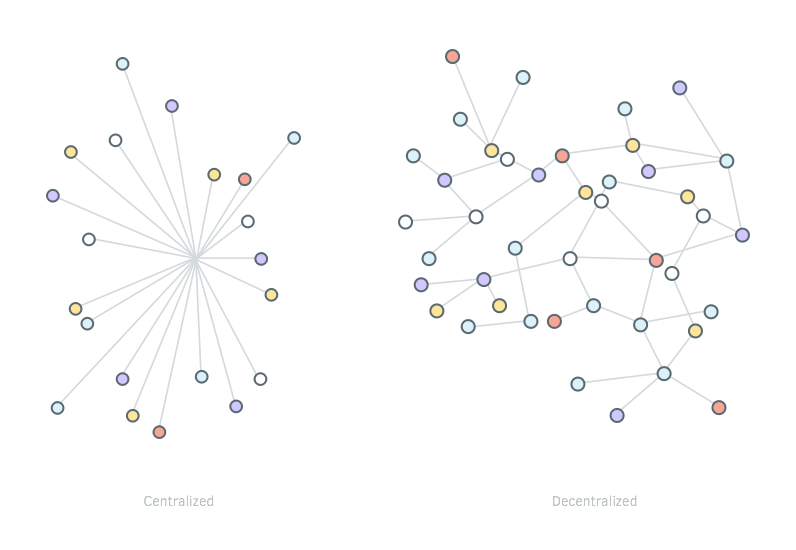
\includegraphics[width=\textwidth]{decentralization.png}
	\caption{Zentrales und dezentrales Netzwerk. Quelle: cryptocoin20.com}
	\label{fig:dencentralized}
\end{figure}

Folgend wird erläutert wie in einer Blockchain die Transaktionen in die Blockchain eingebettet werden. Anschließend wird der Aufbau eines Blockes erläutert. Daraufhin folgt die Erläuterung der Konsensbildung der Blockchain.

\subsection{Transaktionsablauf}
\label{subsec:transaktionsablauf}
Eine Transaktion ist eine Arbeitseinheit, welche eine bestimmte Funktion erf{\"u}llt. In Bezug auf Datenbanksysteme bezeichnet eine Transaktion eine Folge von Datenverarbeitungsbefehlen, die vom System atomar ausgef{\"u}hrt werden.\footnote{\cite[S.~301]{Kemper.2006}} Im Kontext der Blockchain bezeichnet eine Transaktion die Persistierung von Daten, wie beispielsweise einer {\"U}berweisung von Person a zu Person b.\footnote{\cite[S.~2]{SatoshiNakamoto.}} Abbildung \ref{fig:transaktionsablauf} beschreibt den einfachen Transaktionsablauf einer Blockchain.

\begin{figure}[h]
	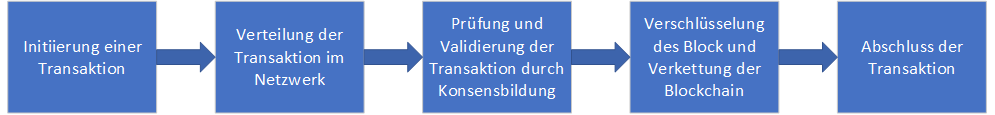
\includegraphics[width=\textwidth]{transaktions-ablauf.png}
	\caption{Vereinfachter Transaktionsablauf. Quelle: Fraunhofer FIT}
	\label{fig:transaktionsablauf}
\end{figure}

Zunächst wird die durchzuführende Transaktion im Netzwerk verteilt. Anschließend fassen die Netzwerkteilnehmer mehrere Transaktionen zu einem Block zusammen und versuchen durch eine Konsensbildung die Transaktionen zu validieren. Die Validierung findet bei der Blockchain-Technologie mit dem sogenannten Proof-Of-Work statt, welche es fordert das aus den Transaktionen und dem vorherigen Block ein Hash mit einer bestimmten Voraussetzung gebildet wird (beispielsweise zehn führende Nullen). Nachdem ein Netzwerkteilnehmer einen validen Hash ermittelt hat, wird der Block an die Kette angehangen und anschließend die veränderte Kette im Netzwerk verteilt. Alle anderen Teilnehmer überprüfen die Erweiterung der Kette mithilfe einer Validierung der Blockhashs. Die Nodes überprüfen auch ob eine Transaktion schon in mehreren Blöcken vorhanden ist oder nicht. Je nach Ergebnis der Validierung wird anschließend die neue Blockchain angenommen oder abgelehnt und die Anpassungen zurückgesetzt.\footnote{\cite[S.~2-4]{SatoshiNakamoto.}}


\subsection{Blockaufbau}
\label{subsec:blockaufbau}
Grundsätzlich besteht ein Block einer Blockchain aus den Transaktionen und Informationen über den aktuellen Block. Mithilfe der Merkle-Root wird aus den einzelnen Transaktionen ein Hashwert ermittelt, jener anschließend in Kombination mit dem vorherigen Blockhash und der freiwählbaren Nonce den Hash des aktuellen Blockes bildet. Mithilfe dieser Einbindung des vorherigen Hash wird die Kette fest miteinander verbunden und die Integrität der Blockchain gewährleistet. In Abbildung \ref{fig:blockaufbau} ist ein Schema der verketteten Blöcke dargestellt.

\begin{figure}[!h]
	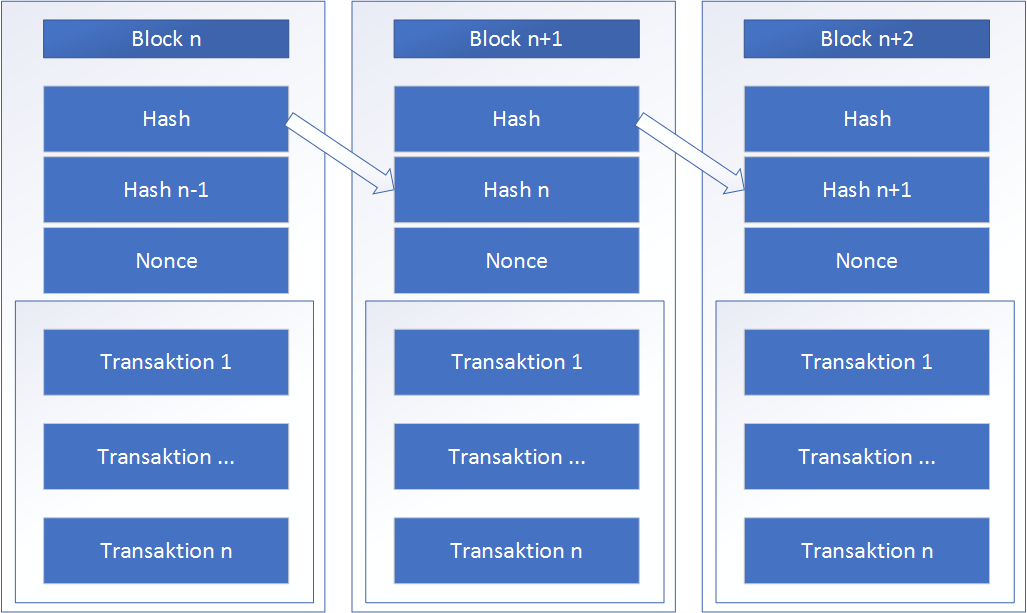
\includegraphics[width=\textwidth]{blockaufbau.png}
	\caption{Blockaufbau. Quelle: Satoshi Nakamoto}
	\label{fig:blockaufbau}
\end{figure}

Die Merkle-Root oder auch Hash-Baum wird für die Sicherstellung der Integrität der Transaktionen verwendet. In Abbildung \ref{fig:hash-tree} ist eine Merkle-Root dargestellt. Zunächst werden alle Transaktionen gehasht. Daraufhin werden zwei gehashte Transaktionen erneut gehasht. Diese Ergebnisse werden anschließend erneut in Zweierpärchen gehasht. Dieser Vorgang wird solange wiederholt, bis nur noch ein Hash übrig ist. Das Ergebnis dieses Verfahren wird als Top-Hash bezeichnet und fließt anschließend in den Blockhash mit ein.\footnote{\cite[S.~4]{SatoshiNakamoto.}}

\begin{figure}[!h]
	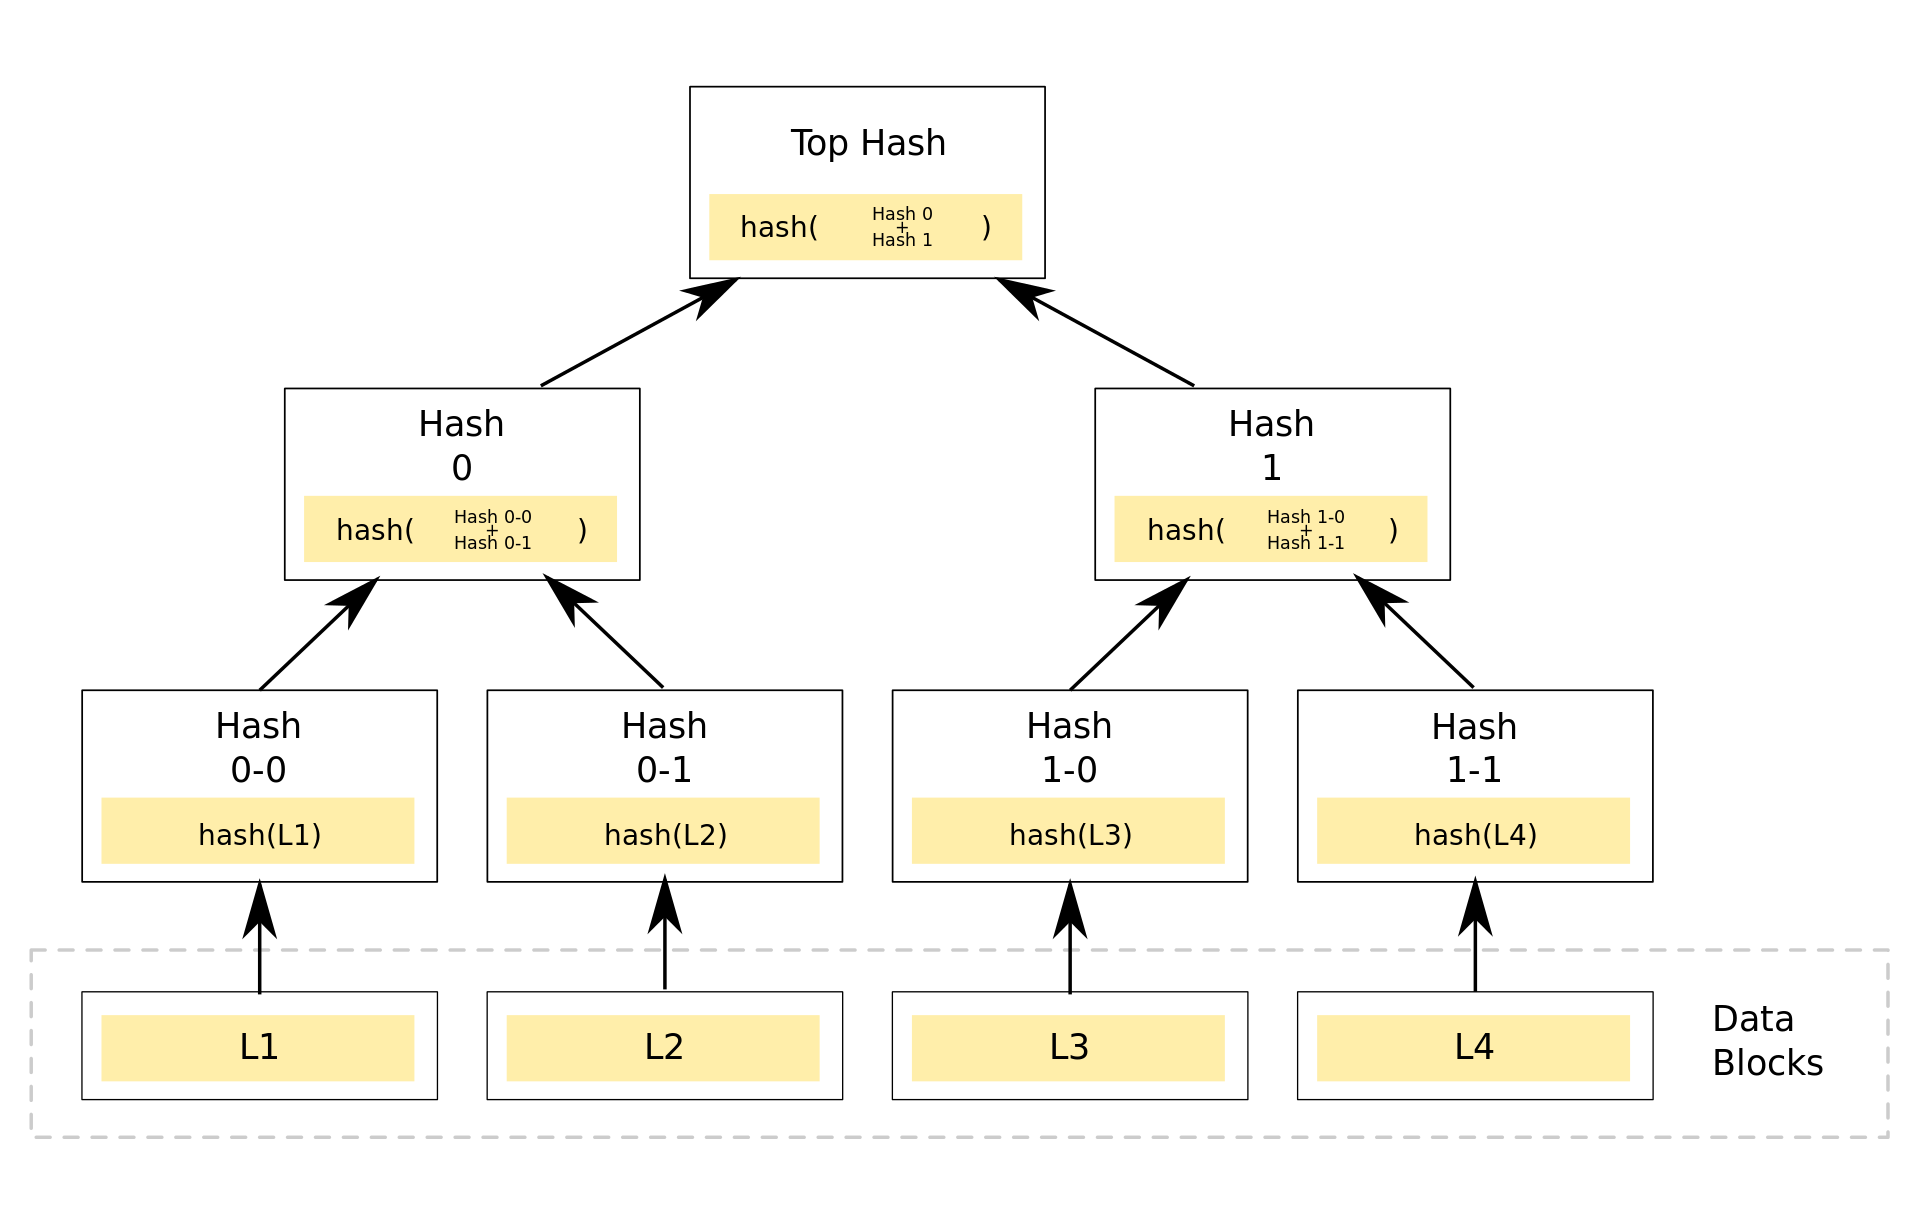
\includegraphics[width=\textwidth]{Hash_Tree.png}
	\caption{Hash-Baum. Quelle: David Göthberg}
	\label{fig:hash-tree}
\end{figure}

\subsection{Konsensbildung}
\label{subsec:Konsensbildung}
Einer der wesentlichen Aspekte des Blockchain-Konzeptes ist die Konsensbildung. Hierbei soll ein Netzwerkteilnehmer beweisen können, dass er berechtigt ist die Blockchain anpassen zu dürfen. Für alle anderen Teilnehmer soll dieser Beweis einfach validierbar sein. Ein weiterer Punkt der Konsensbildung ist die vereinheitlichte Anpassung während der Benutzung der Blockchain. Im den folgenden Kapiteln werden die beiden relevanten Varianten der Konsensbildung vorgestellt.

\subsubsection{Proof-Of-Work}
\label{subsec:proofofwork}
Für Kryptowährungen wird überlicherweise die Proof-Of-Work Variante genutzt. Hierbei muss ein Teilnehmer Arbeit aufwenden, welche anschließend von den anderen Teilnehmern überprüft werden kann.\footnote{\cite[S.~314]{Neugebauer.2018}}

Für die Bitcoin Blockchain müssen beispielsweise Blockhashs mit einer spezifischen Anzahl von führenden Nullen generiert werden. Da eine Hashfunktion eine Einwegfunktion ist, bleibt dem Teilnehmer nichts anderes übrig, als solange den freiwählbaren Teil des Blockes, also den Nonce, anzupassen und anschließend die Hashfunktion auszuführen, bis der gewünschte Hash vorhanden ist.\footnote{\cite[S.~314]{Neugebauer.2018}}

In einer Kryptowährung wie Bitcoin wird in diesem Schritt auch eine Ausschüttung der Währung durchgeführt. Das bedeutet der Teilnehmer, der als erstes die Konsensbildung löst, erhält einen definierten Betrag von der Kryptowährung. Da jedoch mit steigender Nachfrage auch die Anzahl der Netzwerkteilnehmer, bei einer Kryptowährung auch als Miner bezeichnet, steigt, sinkt gleichzeitig die Dauer der Blockerstellung. Um dieser Entwicklung entgegenzuwirken besteht die Möglichkeit die Anforderung an die Konsensbildung regelmäßig zu steigern und somit den steigenden Rechenleistungen entgegenzuwirken.\footnote{\cite[S.~315]{Neugebauer.2018}}

Die Proof-Of-Work Variante ist für öffentliche Blockchains geeignet, da es keine verifizierte Teilnehmer benötigt und trotzdem die Integrität der Blockchain gewährleistet.

\subsubsection{Proof-Of-Stake}
\label{subsec:proofofstake}
Für private Blockchains dagegen ist es nicht immer sinnvoll CPU-Ressourcen für die Konsensbildung zu nutzen. Eine Alternative hierfür wäre das Proof-Of-Stake Verfahren. Hierbei haben einige Nodes besondere Berechtigungen die Blockchain anzupassen und es wird per Zufall ausgewählt, welcher Teilnehmer die Transaktionen an die Blockchain anhängen soll. Die Nodes mit der Berechtigung neue Blöcke an die Blockchain anzuhängen, müssen jedoch in dieser Variante zuvor definiert werden und damit entfällt auch die Unabhängigkeit von einer zentralen Instanz.\footnote{\cite[S.~315--316]{Neugebauer.2018}}

\subsection{Zusammenfassung}
Eine Blockchain ist eine verkette Liste von Blöcken in einem verteilten Peer-To-Peer Netzwerk. Jeder Netzwerkteilnehmer besitzt eine komplette Kopie der Datensätze. Um Daten in das Netzwerk einspeisen zu können, muss der Nutzer eine Transaktion per Broadcast an das Netzwerk senden. Die Netzwerkteilnehmer, auch Nodes genannt, bündeln mehrere Transaktionen und führen je nach Blockchaineigenschaften entweder Proof-Of-Work oder Proof-Of-Stake zur Konsensbildung durch. Hierbei werden zunächst die Transaktionen mithilfe eines Hash-Baums zu einem Hash zusammengefasst. Anschließend wird dieser Hash mit dem Hash des vorherigen Blockes kombiniert. Im Falle der Proof-Of-Work Variante wird danach ein Nonce-Wert gesucht, welcher in Kombination mit den anderen Hashs einen Hash ergibt, der den Ansprüchen der Blockchain genügt. Im Falle der Proof-Of-Stake-Variante wird einfach der Top-Hash der Transaktionen mit dem vorherigen Blockhash kombiniert. Anschließend wird in beiden Verfahren die erweiterte Blockchain im Netzwerk verteilt. Jeder andere Teilnehmer validiert daraufhin die Blockchain.

Da die Blockchain dezentral aufgebaut ist, ergibt sich ein niedriges Ausfallrisiko. Ein weiterer Vorteil der Dezentralität ist das es keine Vertrauensinstanz existieren muss und durch den Proof-Of-Work trotzdem die Integrität der Daten gesichert ist. Eine Blockchain eignet sich aus diesen Gründen für eine öffentliche Währung. Jedoch können Blockchains auch in Unternehmen verwendet werden, da Daten manipulationssicher gespeichert werden können. Diese Eigenschaft könnte beispielsweise in der Rückverfolgung von Lebensmitteln genutzt werden.